\chapter{Analyse Statique : audit d'OpenSSL}

\section{But de cette partie}
Nous nous sommes concentrés sur les parties qui peuvent être critiques : 
\begin{description}
	\item [l'entropie :] un des problèmes les plus épineux lors de la génération de clef ;
	\item [la génération des clefs : ] c'est sur elles que reposent la sécurité d'un système cryptographique. Si leurs secrets venaient à être découverts, un utilisateur malveillant pourrait s'en servir pour déchiffrer facilement les massages d'un tiers (les fonctions de chiffrements étant en théorie publiques et éprouvés) ;
	\item [le chiffrement et les protocoles :] des failles sont trouvées régulièrement dans certains protocoles, et les avancées technologiques tendent aussi à rendre les algorithmes obsolètes (augmentation de la puissance de calcul des machines) ;
	\item [les signatures et les authentifications : ] les certificats et les signatures électroniques ont une importance particulière dans la sécurité protocolaire, et le mécanisme est souvent transparent à l'utilisateur ;
	\item [les protocoles SSL et TLS : ] OpenSSL est basé directement sur le protocole SSL puis ensuite sur celui de TLS (successeur de SSL).\\
\end{description}
Cette deuxième partie est un très court résumé du rapport d'audit réalisé pendant le projet. Pour de plus amples informations, nous vous conseillons de le consulter. Il est accessible sur le site web, onglet "Audit d'OpenSSL", et sur le git \cite{notregit}.

\subsection{Entropie}

L'entropie est la base pour générer des nombres pseudo-aléatoires. Elle joue donc un rôle prépondérant dans la sécurité de la cryptographie qui sera mise en place. Son générateur est composé de trois principaux éléments : 
\begin{description}
	\item [le bruit source : ] il doit être non déterministe, et renvoie de façon aléatoire des bits grâce à des processus non déterministes;
	\item [le composant de conditionnement : ] il permet d’augmenter ou de diminuer le taux d’entropie reçu;
	\item [une batterie de tests : ] elle fait également partie intégrante du système. Des tests sont réalisés pour déterminer l’état de santé du générateur aléatoire, permettant de s’assurer que la source d’entropie fonctionne comme attendu.\\
\end{description}

Plusieurs standards parlent de l'entropie, dont principalement la RFC 4086 \cite{rfc4086} et le FIPS 140 \cite{fips140-1} \cite{fips140-2}. Mais malgré les recommandations, quelques failles ont étés trouvées.\\

\textit{Nous vous invitons à vous référer au rapport d'audit, chapitre 2, pour de plus amples informations} 

\subsection{Génération des clefs}

Les clefs cryptographiques ont un rôle fondamental en cryptographie. En effet, elles sont censées être le seul secret à garder précieusement par leur possesseurs : il est conseillé que les algorithmes et tous les outils ne soient pas secret afin d'être certain de ne pas insérer de faille. Les algorithmes reconnus et éprouvés \textbf{exigent} la fiabilité contrairement aux algorithmes secrets et personnels.\\

Par conséquent les clefs se doivent d'être les plus solides possible. Mais malgré le soin qu'on peut y apporter, et les différentes recommandations qui sont faites par les normes, le risque zéro n'existe pas.\\

\textit{Nous vous invitons à vous référer au rapport d'audit, chapitre 2, pour de plus amples informations} 

\subsection{Chiffrement et protocoles}
De nombreux protocoles de chiffrement existent : 
\begin{itemize}
	\item symétrique :
	\begin {itemize}
		\item AES ;
		\item Blowfish ;
		\item DES ;
		\item 3-DES ;
		\item etc.\\
	\end{itemize}
	\item asymétrique : 
	\begin {itemize}
		\item DSA ;
		\item El Gamal ;
		\item RSA ;
		\item etc.\\
	\end{itemize}
\end{itemize}

RSA étant l'un des algorithmes les plus utilisés en cryptographie asymétrique, et étant limité dans le temps, nous nous sommes concentrés sur celui-ci.\\
Cependant, RSA seul n'est plus d'une sécurité absolue. Il peut-être est combiné par exemple à OAEP (RSA-OAEP). Un bourrage (\textit{padding}) est alors rajouté avant l'application de RSA. La norme principale qui se charge des recommandations sur RSA est la PKCS\#1, qui a aussi le nom de RFC 3447 \cite{3447} \cite{rfc3447_trad}.\\

\textit{Pour plus d'informations, nous vous invitons à aller consulter le rapport d'audit, chapitre 3} 

\subsection{Signature et authentification}
La signature électronique est de plus en plus utilisée, de façon plus ou moins transparente. Un mécanisme complexe est mis en place derrière, avec toute une chaîne d'autorités de certification et de révocation des certificats, ce qui permet de définir le niveau de fiabilité du certificat. \\
Processus de signature : 
\begin{figure}[H]
\begin{center}
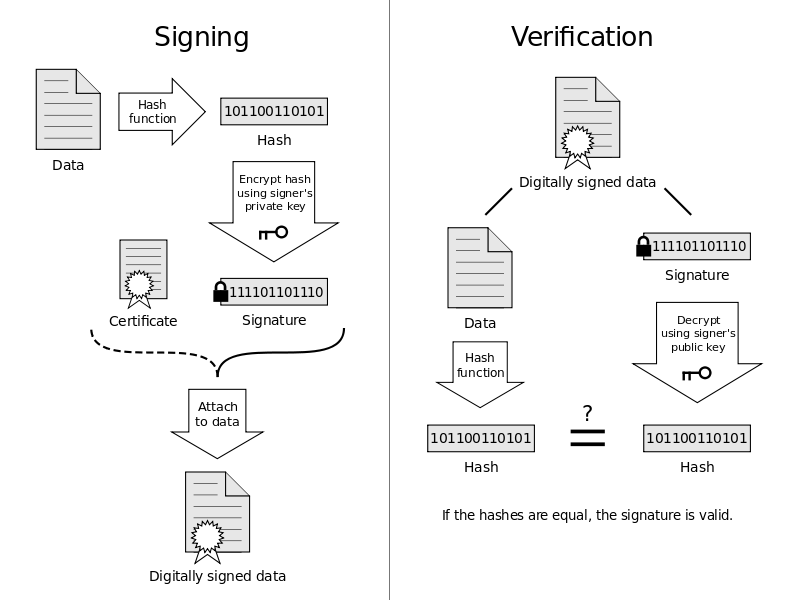
\includegraphics[width=10cm]{images/sig_dig.png}
\end{center}
\caption{Signature électronique}
\label{digital sig}
\end{figure}

La RFC 3447 \cite{rfc3447} \cite{rfc3447_trad} apporte aussi des recommandations à ce propos, ainsi que la RFC 979 \cite{rfc979}.\\

\textit{Pour consulter les principales failles que nous avons trouvées à ce sujet, nous vous invitons à aller consulter le rapport d'audit, chapitre 4} 

\subsection{Protocole SSL/TLS}
SSL et TLS (successeur de SSL) sont des protocoles de sécurisation des échanges sur internet. Les versions 2 et 3 de SSL ont été développées par Netscape puis le brevet a été racheté par l’IETF en 2001, qui a ensuite publié une évolution de ce protocole : TLS. Ce protocole fonctionne selon un mode client-serveur et fournit les objectifs de sécurité suivants :
\begin{itemize}
	\item authentification serveur/client;
	\item confidentialité des données échangées;
	\item intégrité des données échangées.\\
\end{itemize}
Du point de vue réseau, ce protocole se situe dans la couche session du modèle OSI et entre transport et application dans le modèle TCP.\\

\textit{Pour de plus amples informations, nous vous invitons à aller consulter le rapport d'audit, chapitre 5.}



















